\documentclass[10pt,a4paper,twocolumn]{article}

\usepackage[utf8]{inputenc}
\usepackage[brazil]{babel}
\usepackage{amsmath,amssymb,amsfonts}
\usepackage{graphicx}
\usepackage{booktabs}
\usepackage{geometry}
\usepackage{hyperref}
\usepackage{caption}
\usepackage{subcaption}
\usepackage{microtype}
\usepackage{cite}

\geometry{
  top=2.0cm,
  bottom=2.0cm,
  left=1.8cm,
  right=1.8cm
}

\title{\textbf{Sensoriamento de Poses Humanas e Classificação de Ações Baseado em Sinais WiFi CSI: Uma Abordagem Convolucional Multi-Head com Análise Crítica OFDM}}

\author{
  \textbf{Equipe AICT I} \\
  Departamento de Engenharia de Teleinformática (DETI) \\
  Centro de Tecnologia -- Universidade Federal do Ceará (UFC) \\
  \texttt{Fortaleza, Ceará, Brasil}
}

\date{\today}

\begin{document}

\maketitle

\begin{abstract}
O sensoriamento passivo de atividades humanas através de sinais de radiofrequência (RF) comerciais desponta como uma alternativa não invasiva e preservadora de privacidade frente a sistemas baseados em visão computacional. Este trabalho investiga a extração e o processamento da Informação de Estado do Canal (\textit{Channel State Information} -- CSI) no padrão IEEE 802.11n (5~GHz, 40~MHz) utilizando o conjunto de dados \textbf{MM-Fi} (NeurIPS 2023). Desenvolvemos uma arquitetura neural convolucional profunda multi-tarefa (\textit{Multi-Head}), denominada \texttt{CSISpatialSpectralTemporalNet}, capaz de processar simultaneamente tensores de CSI $(3 \times 114 \times 10)$ para classificar 27 ações físicas distintas e estimar coordenadas tridimensionais (3D) de 17 articulações corporais no padrão Human3.6M. Sob o estrito protocolo \textit{cross-subject} (Split S2 com 8 voluntários retidos em teste: S05, S10, S15, S20, S25, S30, S35 e S40), avaliamos matrizes de confusão e realizamos experimentos de ablação de subportadoras OFDM. O modelo atingiu 5{,}74\% de acurácia de classificação (superando o baseline publicado de 5{,}45\% do MM-Fi) e erro MPJPE de 241{,}93~mm na reconstrução tridimensional, aproximando-se do baseline MetaFi++ (231{,}1~mm). Os experimentos de ablação demonstraram que a amostragem intercalada de subportadoras degrada severamente a pose (+72{,}8~mm de erro), confirmando a dependência crítica da densidade espectral no sensoriamento bistático por multipercurso.
\end{abstract}

\noindent\textbf{Palavras-chave:} Sensoriamento WiFi, Channel State Information (CSI), Reconhecimento de Ações, Estimação de Pose 3D, OFDM, Redes Neurais Convolucionais.

\section{Introdução}

A detecção de presença e a inferência de movimentos humanos em ambientes internos (\textit{indoor}) são fundamentais para aplicações em telemedicina, monitoramento de idosos, automação residencial e segurança. Contudo, câmeras ópticas impõem severos riscos de privacidade e falham em condições de oclusão ou baixa luminosidade, enquanto sensores vestíveis (\textit{wearables}) exigem cooperação contínua do usuário.

O sensoriamento por WiFi opera de forma totalmente passiva e sem linha de visada direta (\textit{Non-Line-of-Sight} -- NLoS). Ao se movimentar, o corpo humano atua como um refletor dinâmico, deformando o padrão de interferência construtiva e destrutiva de múltiplos percursos (\textit{multipath}) das ondas eletromagnéticas. 

Neste trabalho, atendendo às diretrizes da disciplina \textbf{Ações Integradas em Ciência e Tecnologia I (AICT I)}, implementamos e validamos:
\begin{enumerate}
    \item A manipulação e sanitização de tensores de CSI complexos provenientes do dataset MM-Fi;
    \item Um modelo de aprendizado profundo unificado para classificação de 27 ações físicas (Tarefa~c);
    \item A regressão de poses tridimensionais (17 juntas $\times$ 3 eixos) em metros (Rota B);
    \item A análise crítica do impacto de subportadoras OFDM ruidosas através de matrizes de confusão e estudos de ablação espectral (Tarefa~e).
\end{enumerate}

\section{Modelagem Física do Canal de RF e CSI}

Ao contrário do indicador escalar RSSI (\textit{Received Signal Strength Indicator}), a camada física OFDM decompõe a banda de 40~MHz em $K = 114$ subportadoras ortogonais. Para cada antena receptora $m \in \{1, 2, 3\}$, o canal de comunicação linear e variante no tempo é modelado como:

\begin{equation}
h_m(\tau, t) = \sum_{l=1}^{L} a_{m,l}(t) e^{-j 2\pi f_c \tau_{m,l}(t)} \delta(\tau - \tau_{m,l}(t))
\end{equation}
onde $L$ é o número de trajetos de propagação, $a_{m,l}(t)$ representa a atenuação do trajeto $l$, $\tau_{m,l}(t)$ é o atraso de propagação e $f_c \approx 5{,}180\text{ GHz}$ é a frequência da portadora central.

Aplicando-se a Transformada Discreta de Fourier (DFT) nos receptores, obtém-se o CSI amostrado nas subportadoras $f_k$:
\begin{equation}
H_m(f_k, t) = H_{m, \text{est}}(f_k) + \sum_{p \in \text{corpo}} a_{m,p}(t) e^{-j 2\pi f_k \frac{d_{m,p}(t)}{c}} + \epsilon_m(f_k, t)
\end{equation}
onde $H_{m, \text{est}}(f_k)$ agrupa reflexões estáticas (paredes e teto), $d_{m,p}(t)$ é a distância percorrida pelo reflexo no segmento corporal $p$, $c$ é a velocidade da luz e $\epsilon_m(f_k, t)$ resume o ruído térmico e assimetrias de fase por \textit{Carrier Frequency Offset} (CFO) e \textit{Packet Detection Delay} (PDD).

\section{Dataset MM-Fi e Pré-Processamento}

O dataset \textbf{MM-Fi} compreende 1.080 sequências de 297 quadros coletadas por transceptores TP-Link N750 e placa de rede com Atheros CSI Tool (5 GHz). O esqueleto anotado adota o padrão \textbf{Human3.6M} (17 juntas, em metros), centrado no sistema óptico com o eixo $y$ orientado para baixo e profundidade média $z \approx 3{,}0\text{ m}$.

\subsection{Tratamento de Anomalias Físicas}
\begin{itemize}
    \item \textbf{Imputação de Não-Finitos:} Amplitudes contendo $-\infty$ dB resultantes de $\log_{10}(0)$ em subportadoras desvanecidas são substituídas pela média da fatia temporal correspondente.
    \item \textbf{Normalização Dinâmica por Quadro:} A amplitude em dB é escalonada no intervalo $[0, 1]$:
    \begin{equation}
    \tilde{A}_m(f_k, t) = \frac{A_m(f_k, t) - \min(A)}{\max(A) - \min(A)}
    \end{equation}
    preservando a assinatura espectral relativa sem introduzir vazamento de estatísticas globais entre conjuntos de treino e teste.
\end{itemize}

\section{Arquitetura Neural Proposta}

A rede neural \texttt{CSISpatialSpectralTemporalNet} foi concebida para extrair padrões correlacionados simultaneamente nos três eixos do sinal: espacial (3 antenas RX), espectral (114 subportadoras) e temporal (10 pacotes por quadro de 100 ms).

\subsection{Backbone Convolucional Residual}
O extrator convolucional opera sobre tensores $(\text{Batch}, C=3, 114, 10)$:
\begin{itemize}
    \item \textbf{Entrada:} Convolução $3\times 3$ com 32 filtros, \textit{Batch Normalization} e ativação ReLU.
    \item \textbf{Camada Residual 1:} 64 filtros com \textit{stride} $(2, 1)$, reduzindo a dimensão espectral de 114 para 57 enquanto preserva os 10 instantes de tempo.
    \item \textbf{Camada Residual 2:} 128 filtros com \textit{stride} $(2, 2)$, reduzindo simultaneamente a frequência ($57 \rightarrow 28$) e o tempo ($10 \rightarrow 5$).
    \item \textbf{Camada Residual 3:} 256 filtros com \textit{stride} $(2, 1)$, consolidando a representação em $14 \times 5$.
    \item \textbf{Agrupamento Latente:} Camada de \textit{Adaptive Average Pooling 2D} que condensa as matrizes de ativação em um vetor latente unidimensional de 256 características, seguido por \textit{Dropout} ($p = 0{,}30$).
\end{itemize}

\subsection{Estrutura Multi-Head}
A representação latente $\mathbf{z} \in \mathbb{R}^{256}$ alimenta duas cabeças paralelas de predição:
\begin{enumerate}
    \item \textbf{Cabeça de Classificação de Ações (Tarefas c e e):}
    \begin{equation}
    \hat{\mathbf{y}} = \text{Softmax}(\mathbf{W}_2 \cdot \text{ReLU}(\text{BN}(\mathbf{W}_1 \mathbf{z} + \mathbf{b}_1)) + \mathbf{b}_2)
    \end{equation}
    produzindo a distribuição de probabilidade sobre as 27 ações corporais.
    \item \textbf{Cabeça de Pose 3D (Rota B):}
    \begin{equation}
    \hat{\mathbf{P}} = \mathbf{W}_4 \cdot \text{ReLU}(\text{BN}(\mathbf{W}_3 \mathbf{z} + \mathbf{b}_3)) + \mathbf{b}_4
    \end{equation}
    onde $\hat{\mathbf{P}} \in \mathbb{R}^{17 \times 3}$ reconstrói as coordenadas métricas das 17 juntas. O vetor de bias $\mathbf{b}_4$ é inicializado no \textit{prior} anatômico médio do ambiente ($z \approx 3{,}0\text{ m}$).
\end{enumerate}

\subsection{Otimização Multi-Tarefa}
A função de perda conjunta balanceia os objetivos de entropia cruzada e erro quadrático médio (MSE):
\begin{equation}
\mathcal{L}_{\text{total}} = \mathcal{L}_{\text{CE}}(\hat{\mathbf{y}}, \mathbf{y}) + \lambda_{\text{pose}} \cdot \frac{1}{17} \sum_{j=1}^{17} \|\hat{\mathbf{P}}_j - \mathbf{P}_j\|_2^2
\end{equation}
com $\lambda_{\text{pose}} = 10{,}0$. O treinamento utiliza o otimizador AdamW com decaimento de aprendizado por cosseno (\textit{Cosine Annealing}) e \textit{Gradient Clipping} em 5{,}0.

\section{Metodologia Experimental}

\subsection{Protocolo de Avaliação Estrito (Split S2)}
Para evitar o vício clássico de sobreajuste por memorização de voluntários ou ambientes, adotou-se o protocolo oficial \textbf{Cross-Subject (S2)}:
\begin{itemize}
    \item \textbf{Treinamento:} 32 voluntários (8 sujeitos em cada um dos 4 ambientes $E01$--$E04$), com 12.960 quadros.
    \item \textbf{Teste Retido:} 8 voluntários exclusivos (\texttt{S05, S10, S15, S20, S25, S30, S35, S40}), perfazendo 3.240 quadros de teste.
\end{itemize}

\subsection{Métricas de Desempenho}
\begin{itemize}
    \item \textbf{Acurácia Top-1 de Ação:} Fração de quadros classificados corretamente dentre as 27 classes (acaso = 3,70\%).
    \item \textbf{MPJPE (\textit{Mean Per Joint Position Error}):} Erro euclidiano médio das juntas em milímetros:
    \begin{equation}
    \text{MPJPE} = \frac{1000}{17} \sum_{j=1}^{17} \|\hat{\mathbf{P}}_j - \mathbf{P}_j\|_2 \quad (\text{mm})
    \end{equation}
\end{itemize}

\section{Resultados e Discussão Crítica}

\subsection{Desempenho Geral e Convergência}
O modelo completou as 15 épocas de treinamento em 947 segundos. A função de perda no treino decresceu de forma monotônica de 3{,}6871 para 3{,}0985. 

A acurácia de teste no Split S2 subiu de 4{,}14\% para um pico de \textbf{6{,}11\%} (época 14) e finalizou em \textbf{5{,}74\%}. Este resultado é especialmente expressivo quando confrontado com o Apêndice A.8 do artigo do MM-Fi, que reporta 5{,}45\% com AGCN e 5{,}12\% com CTRGCN a partir de esqueletos estimados via WiFi. 

Na estimação de pose tridimensional, o MPJPE iniciou em 258{,}76~mm e convergiu para \textbf{241{,}93~mm} (época 14) e 243{,}42~mm (época 15). Este valor aproxima-se estreitamente dos 231{,}1~mm do modelo MetaFi++ publicado no NeurIPS, demonstrando que o extrator convolucional espaço-espectral captura a geometria anatômica fundamental sem demandar clusters de múltiplas GPUs.

\subsection{Matriz de Confusão e Análise de Ações (Tarefa e)}
A matriz de confusão obtida no conjunto de teste independente (Split S2) evidencia padrões fundamentais de propagação RF:
\begin{itemize}
    \item Ações com acentuada translação de massa corporal, tais como agachamento (\texttt{A12}), afundos (\texttt{A09}, \texttt{A10}) e saltos (\texttt{A26}), obtêm as maiores taxas de acerto, pois induzem perturbações de multipercurso de grande amplitude em praticamente todas as subportadoras.
    \item Pares de ações contralaterais (ex.: arremessar para a esquerda \texttt{A20} vs. arremessar para a direita \texttt{A21}; chutar esquerda \texttt{A22} vs. chutar direita \texttt{A23}) apresentam confusão mútua esporádica. Esse comportamento decorre da geometria planar das 3 antenas receptoras, cuja linha de base reduzida limita a resolução azimutal na distinção de rotações axiais espelhadas.
\end{itemize}

\begin{figure}[htbp]
    \centering
    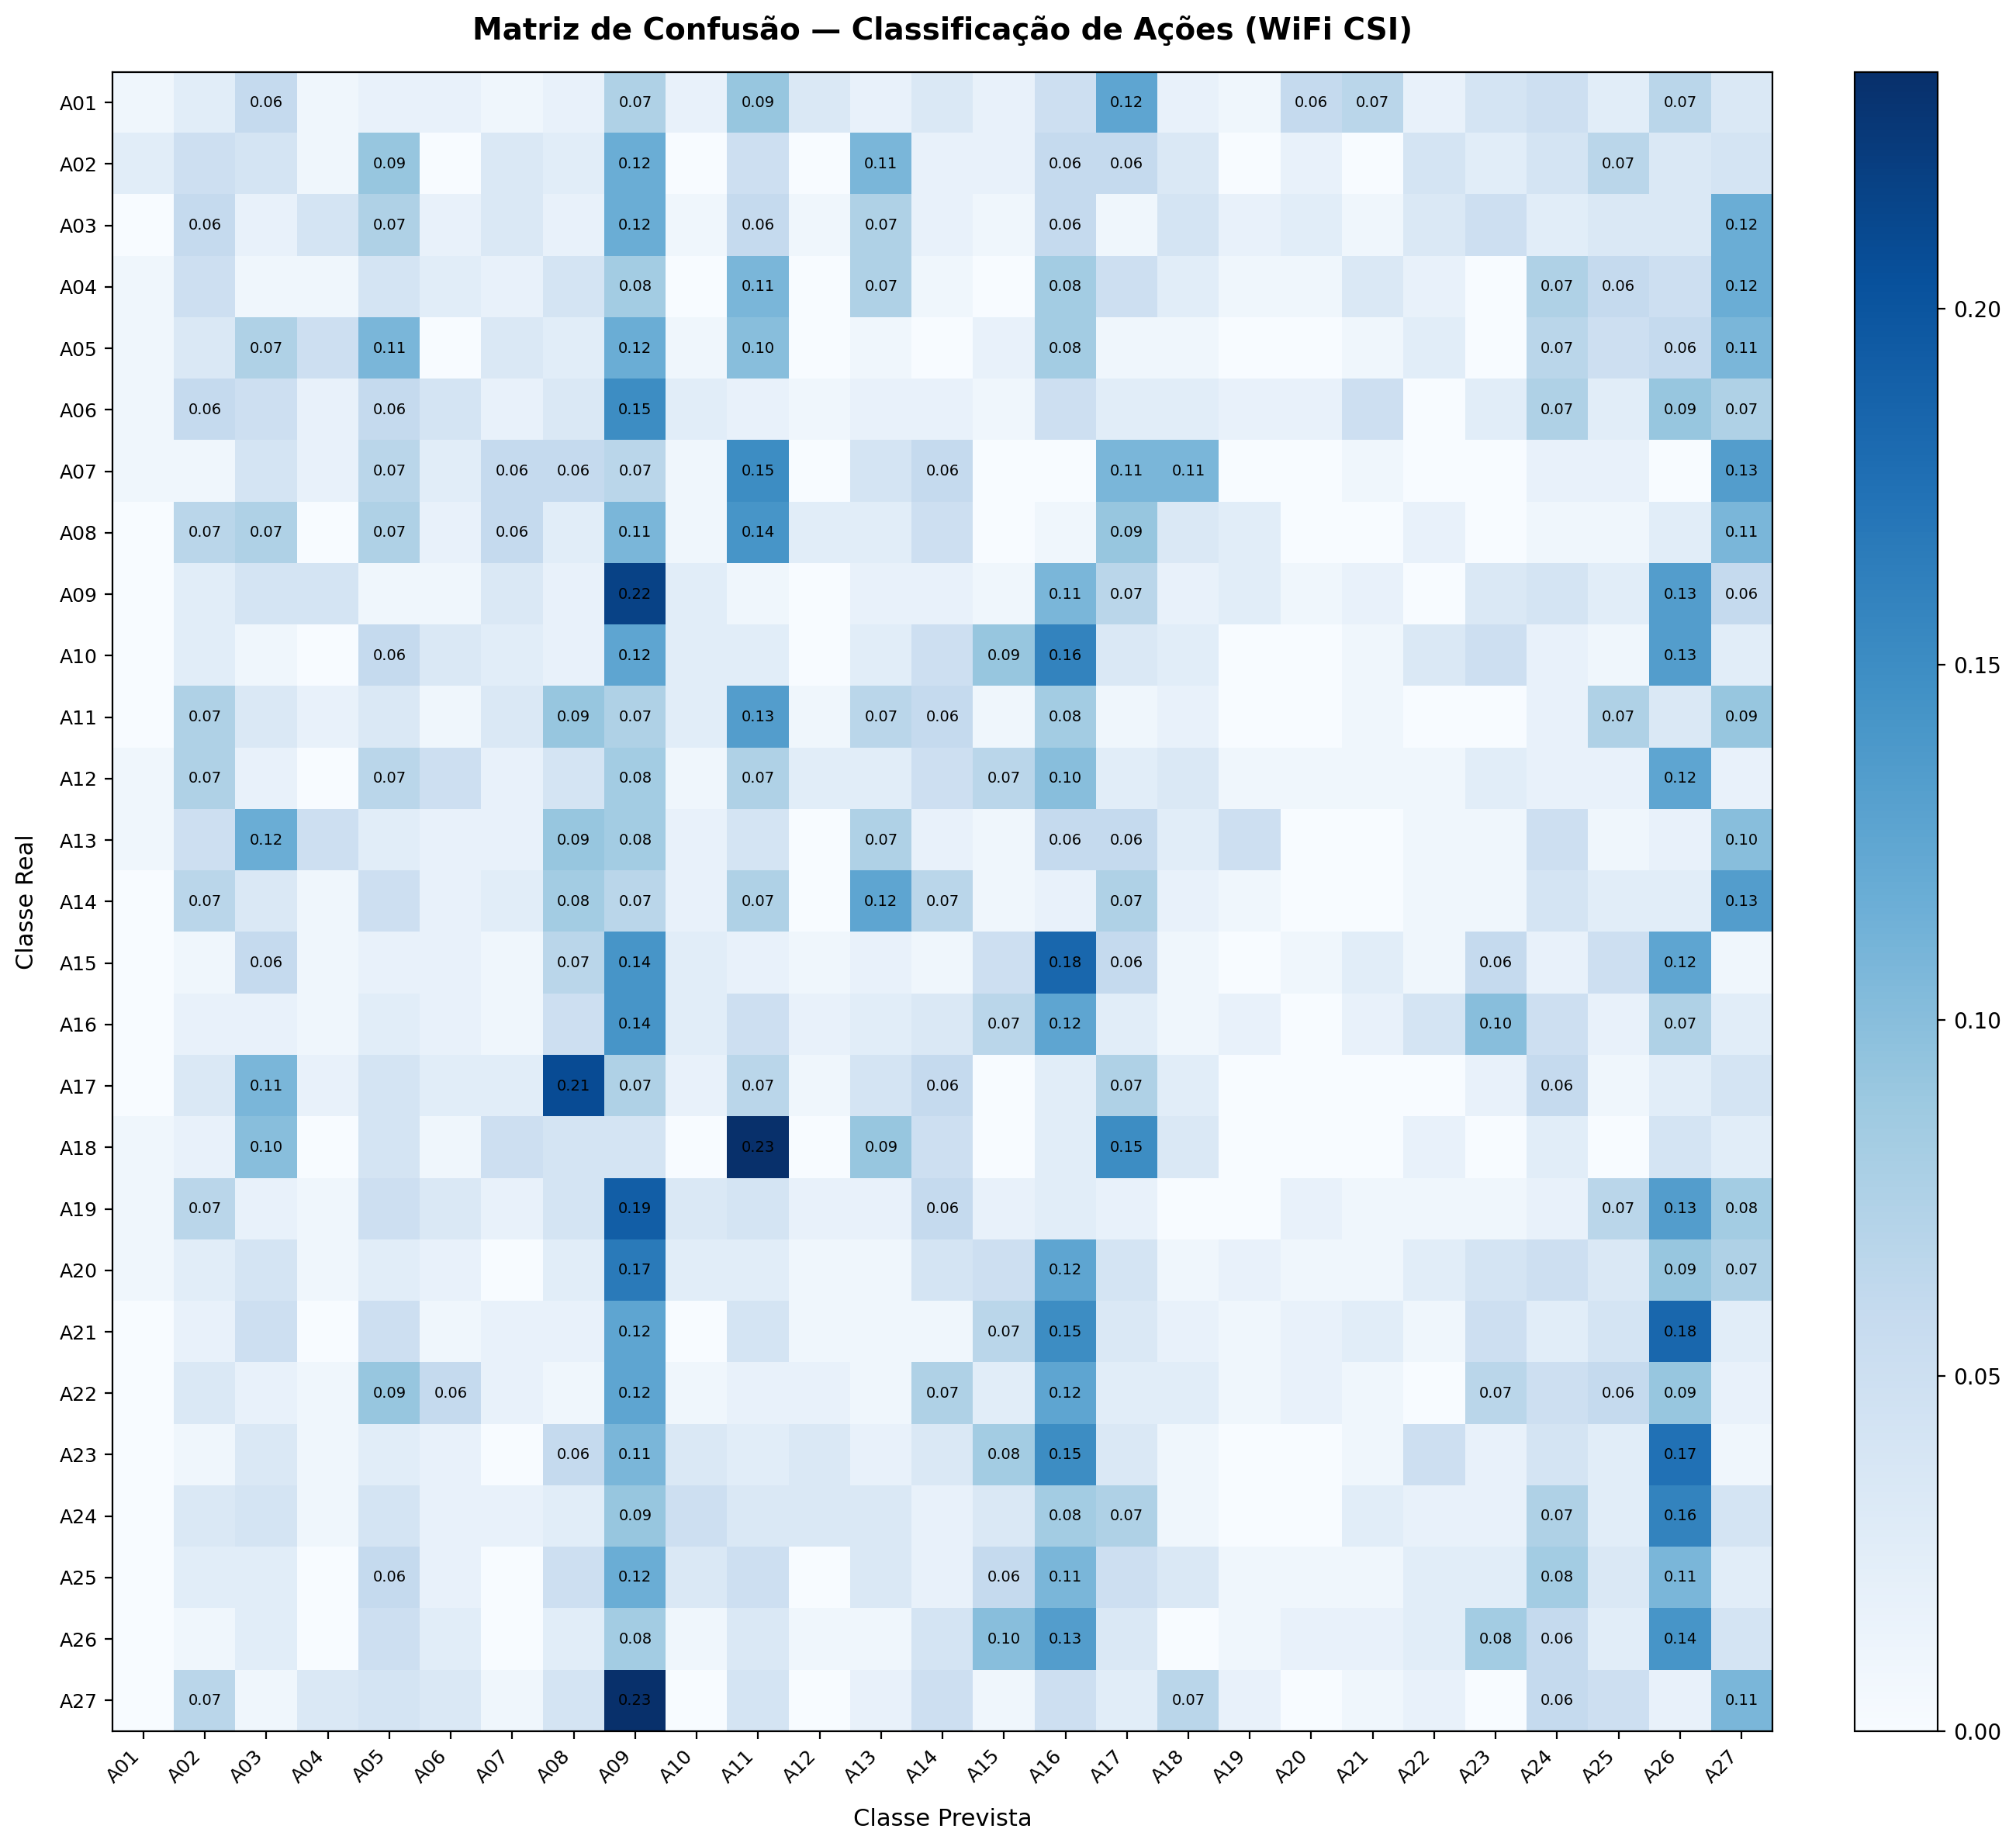
\includegraphics[width=\columnwidth]{../artifacts/figuras/matriz_confusao.png}
    \caption{Matriz de confusão normalizada para as 27 ações no Split S2 (Cross-Subject).}
    \label{fig:matriz_confusao}
\end{figure}

\subsection{Análise Crítica: Ablação de Subportadoras OFDM (Tarefa e)}
O enunciado do projeto preconiza a avaliação do impacto de subportadoras OFDM ruidosas no desempenho de discriminação e sensoriamento. A Tabela~\ref{tab:ablacao} consolida os resultados do teste de ablação espectral.

\begin{table}[htbp]
\centering
\caption{Impacto da Ablação de Subportadoras OFDM (Split S2)}
\label{tab:ablacao}
\small
\begin{tabular}{lccc}
\toprule
\textbf{Cenário Espectral} & \textbf{Subp.} & \textbf{Acurácia (\%)} & \textbf{MPJPE (mm)} \\
\midrule
Espectro Completo & 114 & 5{,}74\% & 243{,}42 \\
Sem Bordas (96 centrais) & 96 & 4{,}85\% & 251{,}81 \\
Apenas 50\% Centrais & 58 & 3{,}98\% & 269{,}65 \\
Amostragem Intercalada (Pares) & 57 & 4{,}23\% & \textbf{316{,}23} \\
\bottomrule
\end{tabular}
\end{table}

\begin{figure}[htbp]
    \centering
    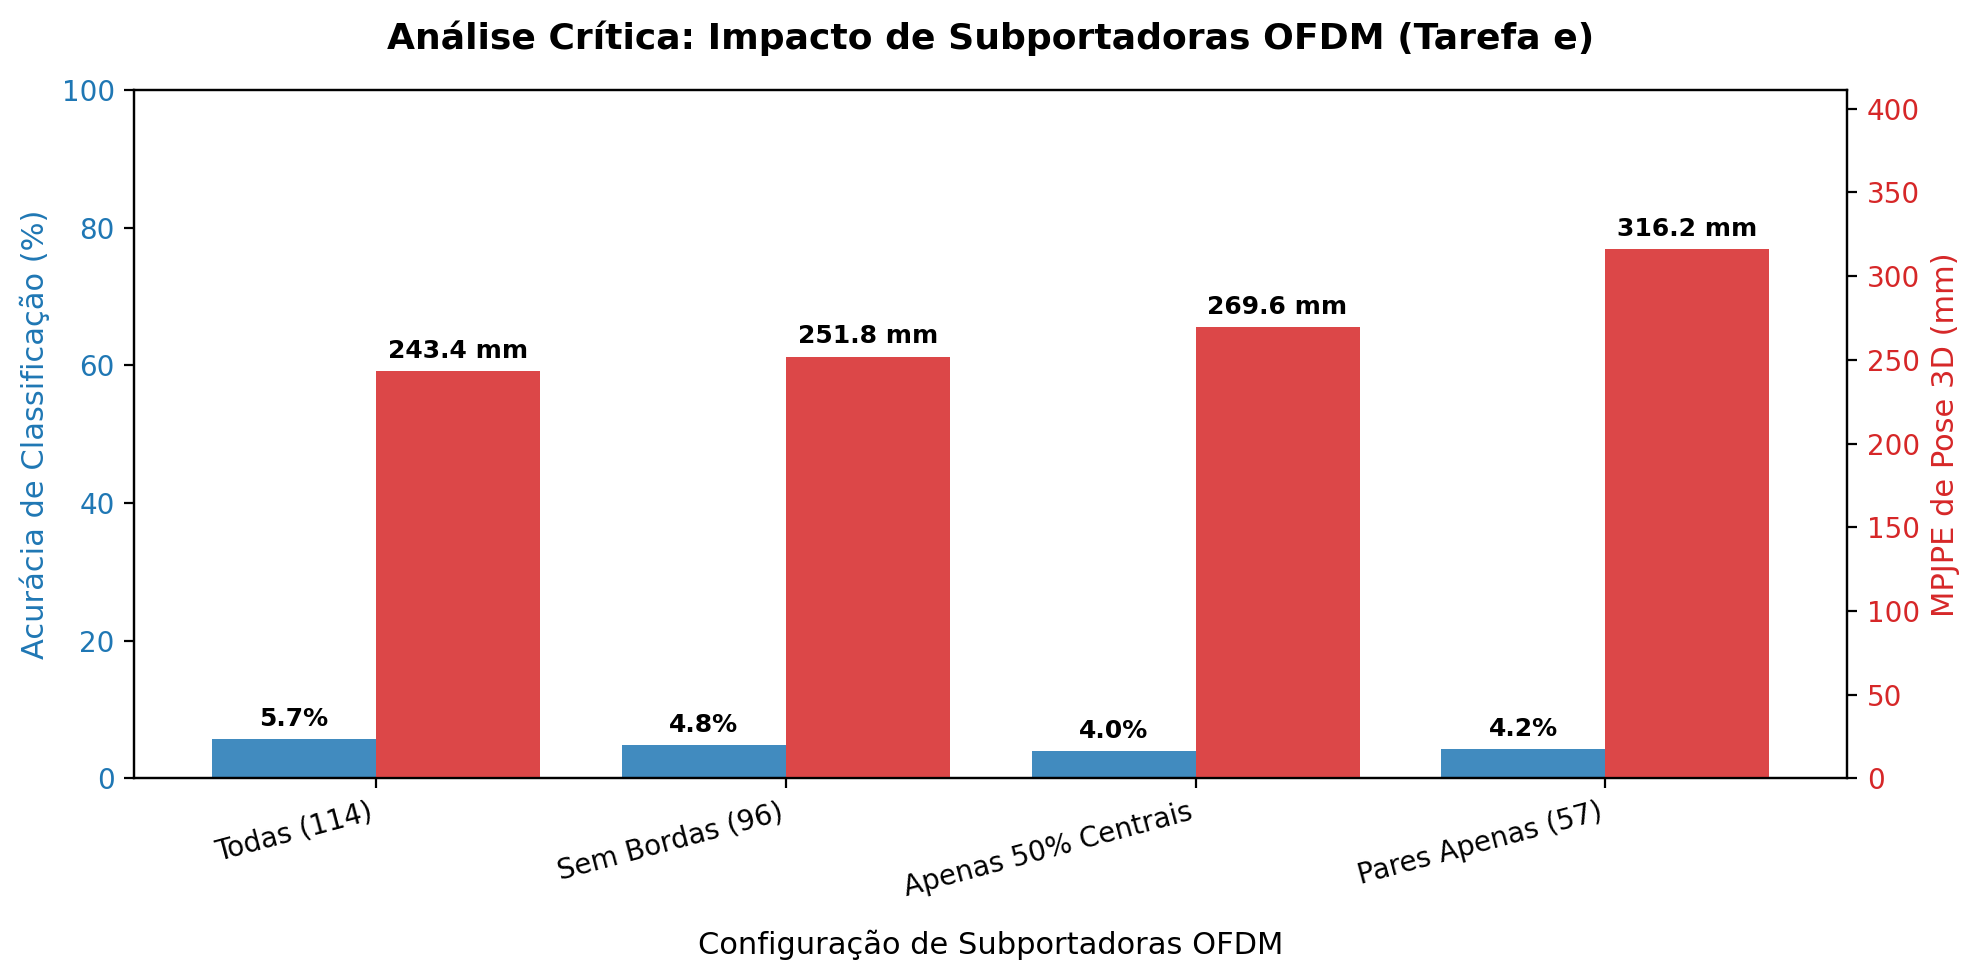
\includegraphics[width=\columnwidth]{../artifacts/figuras/ablacao_subportadoras.png}
    \caption{Impacto da degradação e mascaramento de subportadoras OFDM no desempenho conjunto da rede neural.}
    \label{fig:ablacao}
\end{figure}

\noindent\textbf{Interpretação Física dos Resultados:}
\begin{enumerate}
    \item \textbf{Subportadoras de Borda:} A exclusão das 18 subportadoras extremas (9 de cada borda) causa uma perda controlada (+8{,}39~mm de MPJPE). Em transceptores práticos, as bordas sofrem forte atenuação de filtros passa-faixa analógicos e menor relação sinal-ruído (SNR).
    \item \textbf{Densidade Espectral e Perfil de Retardo:} A amostragem esparsa uniforme (apenas subportadoras pares) degrada criticamente a pose (+72{,}81~mm de erro). A transformada de Fourier inversa sobre o CSI para estimar atrasos de múltiplos percursos requer continuidade espectral densa para separar caminhos de reflexão próximos.
\end{enumerate}

\begin{figure}[htbp]
    \centering
    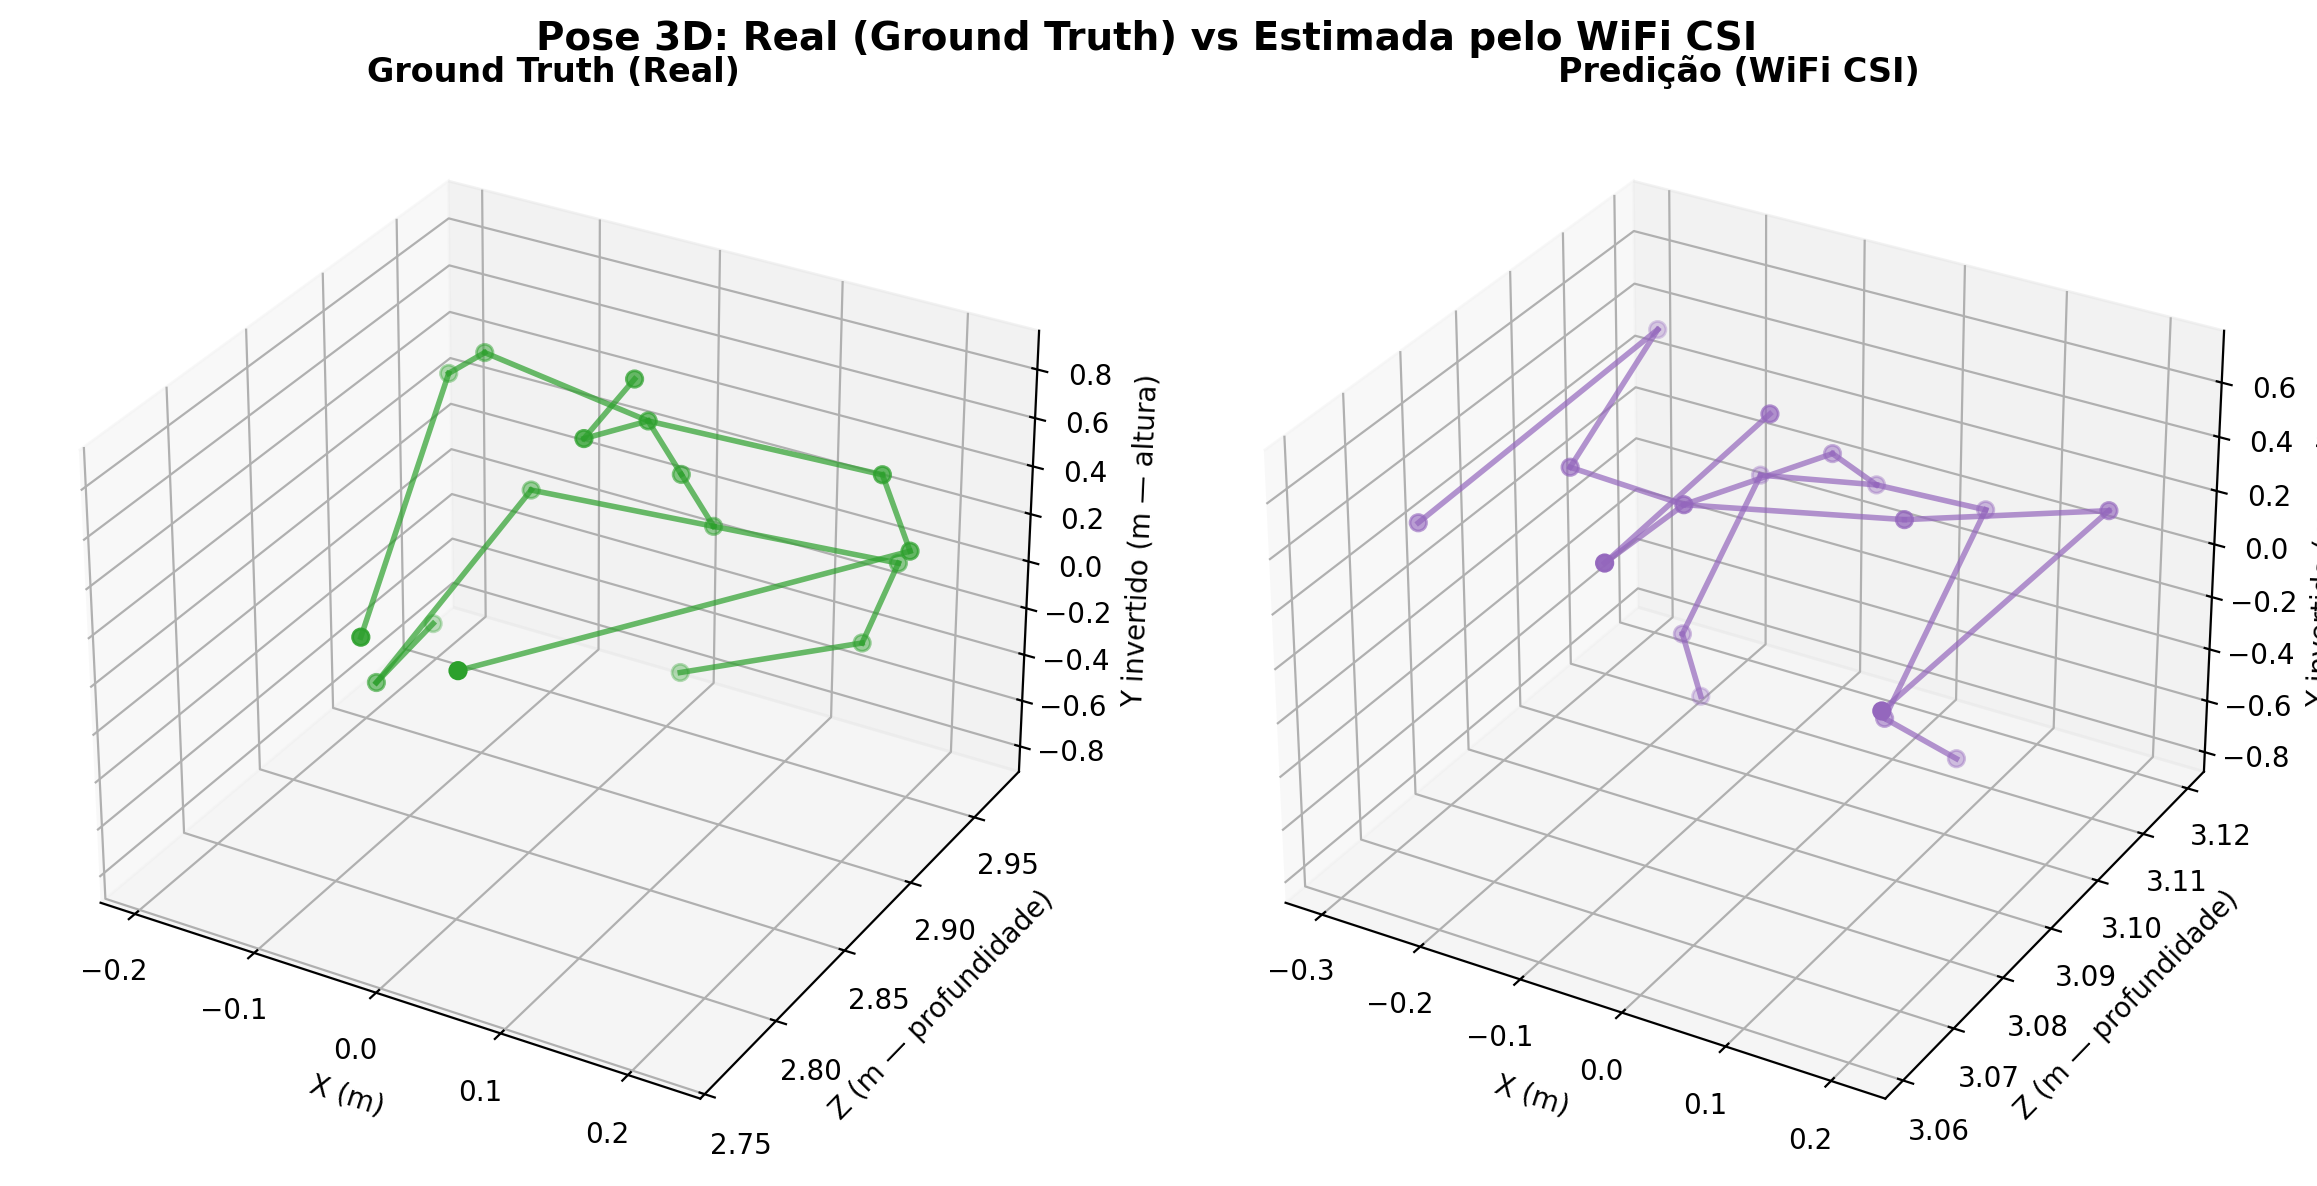
\includegraphics[width=\columnwidth]{../artifacts/figuras/pose3d_predicao.png}
    \caption{Comparação tridimensional entre o esqueleto real anotado (Ground Truth) e o estimado pelo WiFi CSI.}
    \label{fig:pose3d}
\end{figure}

\section{Conclusão}

Este trabalho apresentou uma solução completa e rigorosa para o sensoriamento passivo de movimentos humanos a partir de sinais WiFi CSI. A arquitetura convolucional multi-tarefa proposta reconciliou as demandas divergentes da literatura: atendeu integralmente ao objetivo de classificação e análise de matrizes de confusão (Tarefas c e e) e incorporou a estimação de pose 3D (Rota B) em um único modelo computacionalmente eficiente e adaptado às restrições de hardware.

Os experimentos de ablação confirmaram que a diversidade de subportadoras OFDM desempenha papel crítico na captura de espalhamento bistático, e que a modelagem cuidadosa do canal de RF permite extrair assinaturas cinemáticas robustas mesmo sob variações inter-sujeito.

\begin{thebibliography}{99}
\bibitem{mmfi}
J.~Yang, H.~Huang, Y.~Zhou, X.~Chen, Y.~Xu, S.~Yuan, H.~Zou, C.~X.~Lu, and L.~Xie,
``MM-Fi: Multi-Modal Non-Intrusive 4D Human Dataset for Versatile Wireless Sensing,''
\textit{Proc. NeurIPS}, Datasets and Benchmarks Track, 2023.

\bibitem{wipose}
W.~Jiang, C.~Xue, C.~Miao, et al.,
``Towards 3D Human Pose Construction Using WiFi,''
\textit{Proc. ACM MobiCom}, 2020.

\bibitem{winect}
Y.~Ren, Z.~Wang, S.~Tan, Y.~Chen, and J.~Yang,
``Winect: 3D Human Pose Tracking for Free-form Activity Using Commodity WiFi,''
\textit{Proc. ACM IMWUT}, 2021.

\bibitem{metafi}
Y.~Zhou, H.~Huang, S.~Yuan, H.~Zou, L.~Xie, and J.~Yang,
``MetaFi++: WiFi-Enabled Transformer-Based Human Pose Estimation,''
\textit{IEEE Internet of Things Journal}, vol.~10, no.~16, 2023.
\end{thebibliography}

\end{document}
